\section{The Cosmological Context of Galaxy Formation} The modern picture of
galaxy formation sits within the context of a $\Lambda$ Cold Dark Matter
($\Lambda CDM$) cosmology \citep{Rees1977,White1978,Blumenthal1984,Mo1998}.
This is a universe which has a no curvature ($\Omega = 1$), and today has the
majority of its mass-energy in dark energy $\Lambda$ ($\Omega_\Lambda =
0.6911\pm0.0062$), and most of its matter in a collisionless form (dark matter)
($\Omega_m = 0.3089\pm0.0062$) \citep{Planck2015b}.  Roughly $5\%$ of the
matter-energy density of the universe exists as baryons ($\Omega_b =
0.048613\pm0.00031$).  The composition of the universe, and the precise value of
the mass-energy density for these components sets the lifetime of the universe,
how rapidly it expands (or contracts), and exactly determines the growth of
large-scale structure.  Within this structure is ultimately where galaxies will
form.  All of this began $13.799\pm0.021$ billion years ago \citep{Planck2015b},
with the universe emerging from a state of high temperature and density,
expanding to form what we see today.  The primordial elemental abundances, with
$\sim4/5$ of the universe's baryons in hydrogen, and the remainder in helium,
were established just a few minutes after the big bang, during a brief period of
``Big Bang Nucleosynthesis'' \citep{Alpher1948}.  The remaining heavier elements
have been formed via stellar nucleosynthesis, through fusion in the cores of
stars and in energetic processes that take place during supernovae (SN)
\citep{Wagoner1967}, or through the capture of high energy cosmic ray protons
and $\alpha$ particles by carbon, nitrogen, or oxygen nucleii
\citep{Reeves1970}.  The chemical composition of the universe establishes the
kinds of stars that form within galaxies and the rates at which gas within the
interstellar medium (ISM) and beyond cools.

Much of what we know about the cosmology of our universe comes from observations
of the first light to escape the universe's surface of last scattering as it
became optically thin: the cosmic microwave background radiation (CMB).  
When the CMB was emitted, the baryons of the universe were in the form of a
nearly isothermal ($\delta T/T\sim10^{-5}$) gas of hydrogen and helium.  Prior
to a redshift of $z\approx1100$, the universe had a high ionization fraction
such that the mean free path for photons was short, making all of space
effectively opaque.  Once the universe became cool enough that hydrogen became
fully neutral, the optical depth fell low enough that photons could free-stream,
decoupled from baryons.  We observe this ultraviolet light today, redshifted to
microwaves with a temperature of $2.729\pm0.004\;\rm{K}$ \citep{Fixsen1996}.
When the power spectrum of this radiation is measured \citep{Spergel2003},
features in that spectrum can be used to determine the components of the
universe (with some degeneracy that can be resolved via SN Ia and large scale
structure measurements
\citealt{Riess1998,Perlmutter1999,Beutler2011,Blake2011}). These features also
reveal the spectrum of density perturbations that will eventually form galaxies
\citep{Press1974,Peebles1980}.   The CMB is the single most important
observational tool for understanding the cosmology of our universe.

The formation of structure within the universe began with the gravitational
collapse of small, linear density perturbations seeded by quantum fluctuations
amplified by inflation \citep{Guth1981,Linde1982}.  These perturbations grow
through gravitational collapse.  Until $z\sim1100$, only dark matter
perturbations were able to grow.  Prior to this, baryons were coupled to
photons, causing density perturbations to oscillate as stable sound waves.  This
early collapse of matter meant that when decoupling occurred at $z\sim1100$,
baryons were able to collapse into the deeper potential wells grown out of
dark-matter density perturbations.  These overdensities expand slower that the
surrounding medium, as they experience a drag from their own self-gravity.
Eventually, these regions stop expanding and begin collapsing at the turnaround
time $t_{turn}$, and virialize at roughly $2\;t_{turn}$ \citep{Peebles1980}.
The first galaxies likely began to form around $z\sim20-50$, with minimum sizes
set by the baryonic physics of Silk damping and radiative cooling
\citep{Silk1968}.  Without the earlier growth of dark matter perturbations,
structure formation would have occurred much later, and the number of galaxies
and distribution of their masses would be different than those we see today
\citep{Davis1985}.

The density perturbation spectrum describes the complete statistics of the
Gaussian random field from which structure forms. \citet{Press1974} were able to
show this produces a halo mass spectrum at a given time with a form that matched
the functional form for the observed galaxy mass function
\citet{Schechter1976}:
\begin{equation}
    \frac{dn}{dM}(M,t) =
    \sqrt{\frac{2}{\pi}}\frac{\rho_0\delta_c(t)}{M^2\sigma(M)} 
    \left\lvert\frac{d\ln{\sigma}}{d\ln{M}}\right\rvert
    \exp{\left[-\frac{\delta^2_c(t)}{2\sigma^2(M)}\right]}
\end{equation}
In this equation, $\rho_0$ is the mean density of the universe, and
$\delta_c(t)$ is the critical overdensity for collapse at a given time $t$.  The
mass variance spectrum, $\sigma^2(M)$ can be determined observationally using
the CMB power spectrum \citep{Fixsen1996,Spergel2003,Planck2015} and an
assumption of a specific cosmology.  This function gives an approximate
distribution of masses for the dark matter halos that galaxies will begin to
form within.  As these halos collapse, non-linear gravitational tugs from their
surroundings will impart torques on them \citep{Barnes1987}, causing halos to
have a distribution of angular momenta.  High resolution N-body simulations have
found that dark matter halos have both a universal density profile
\citep{Navarro1996,Merritt2006} as well as a universal angular momentum profile
\citep{Bullock2001}.  These dark matter halos serve as the environment in
which the collapse of baryons and formation of stars take place, fed by
accretion along large-scale filaments.

The collapse of baryons within halos will depend strongly on whether the
post-virialized gas can cool radiatively \citep{Rees1977}.  As gas accretes onto
a halo with overdensity $\Delta$ it collisionally converts its potential energy
into heat, with a characteristic virial temperature:
\begin{equation}
    T_{virial} = \frac{2}{3}\frac{G\mu m_H}{k_B}\left({\frac{4\pi\rho_0\Delta
    M^2}{3}}\right)^{1/3}
\end{equation}
This means that more massive halos have larger virial temperatures, and,
depending on the mode of radiative cooling (atomic cooling from primordial
hydrogen, molecular hydrogen cooling, or cooling through metal lines), this may
give cooling times shorter than the current age of the universe.  These halos
are the ones in which galaxy formation may begin, as their hot gaseous halos can
collapse to form a central concentration where star formation can occur.  In
some halos, virial shocks may be unstable to cooling, allowing the direct
collapse of cold gas onto the disc \citep{Birnboim2003}.  


As gas does begin to cool within these halos, it will lose pressure support (by
radiating away thermal energy), but {\it not} angular momentum.  For large
spiral galaxies, this means that the baryons, which typically carry the same
specific angular momentum as the halo itself, will flatten to form an
exponential disc as they cool \citep{Fall1980,Mo1998}.    A combination
of heating and cooling processes will render this gas multiphase, containing
both warm/hot ($T>10^4\;\rm{K}$) and cold ($T\sim10-100\;\rm{K}$) gas in
quasistatic equilibrium \citep{McKee1977}.  This multiphase state is highly
dependent on both the metallicity and the local heating rates (which
themselves can vary with redshift) \citep{Field1969,Wolfire1995,Norman1997}.  In
the disc of the galaxy, this dense multiphase gas forms the ISM from which stars
collapse and are born.

The formation of stars has a dramatic impact on the galaxy.  As molecular clouds
begin to construct O/B stars with masses $>5\Msun$, these stars immediately
begin to obliterate the clouds from which they form.  A typical $10^5\Msun$
cluster will have an ionizing UV luminosity of $\sim10^5\Lsun$ during its first
few Myr of life.  This UV flux ionizes the surrounding gas, heating it to
$\sim10^4\;\rm{K}$ \citep{Dale2005,Murray2011}.  Along with ionizing radiation,
massive stars drive fast $v>10^3\kms$ stellar winds, further shocking and
destroying the cold, dense gas which stars form from.  By the time the most
massive stars reach the end of their short lives, $\sim4$ Myr later, they
detonate as core-collapse supernovae not in dense ($n>100\hcc$) clouds, but in
their significantly more diffuse remnants \citep{Rogers2013}.  The longer
cooling times this results in allows supernovae to expand through the ISM,
driving turbulance \citep{Ostriker2010} and filling most of the volume with hot,
diffuse gas.  Much of this hot gas is in fact able to leave the ISM, driven out
as hot, buoyant, high-entropy gas.  These feedback-driven outflows remove gas
from the disc, slowing the rate of star formation, and polluting the
intergalactic medium with metals from stellar ejecta.  In the most massive
galaxies ($M>10^{12}\Msun$), these outflows can be driven by the accretion
luminosity of the central supermassive black hole (SMBH).  These Active Galactic
Nuclei (AGN) are observed in giant elliptical galaxies, and can be seen blowing
hot bubbles within the intracluster medium of nearby galaxy clusters.  Further
discussion on feedback can be found in section~\ref{intro:fb}.

\begin{figure}
    \includegraphics[width=0.7\textwidth]{mass_function.eps}
    \caption[Galaxy mass function]{The observed mass function for galaxies in
    the nearby universe (derived using abundance matching for the solid line and
    semi-analytic modelling for the green points) does not match the mass
    function for dark matter halos given in equation 1, scaled by the baryon
    fraction (dashed line).  This tells us that there are additional physical
    processes involved in the formation of galaxies within their dark matter
    halos.  The most likely candidate for this is feedback from stars and black
    holes.  Of particular interest is the peak in star formation efficiency near
    $M_{200}=10^{12}M_\odot$.  \textit{Image credit: Adapted from figure 1 in
    \citet{Ferrero2012}}}.
\end{figure}

These are of course all highly idealized, simple models for the broadest strokes
of galaxy formation.  Each of these halos will begin to undergo mergers and
interactions \citet{Navarro1993,Kauffmann1999,Cole2000} with each other that can
strip stars and gas through tidal and ram pressure forces
\citep{Gunn1972,Dressler1980}.  Inside each of these halos, the process of disc
collapse, the formation of a multiphase ISM, star formation, and feedback from
those stars involves the complex, nonlinear interplay of radiation,
hydrodynamics, magnetic fields, and gravity on length scales as much as
$10^{11}$ times smaller than the virial radius.  None of this physics is simple
enough to be fully captured by analytic models. As figure 1.1 shows, the
observed mass function for galaxies does not match what would be expected from
the total baryon budget for each halo, implying that at least some of these
processes must change the galactic star formation efficiency as a function of
halo mass, establishing the population of galaxies we see today.  Numerical
simulations have therefore become a keystone for galaxy formation research.


\section{Numerical Simulations of Galaxies}
N-body Simulations of galaxies actually predate {\it digital} simulations of
galaxies.  \citet{Holmberg1941} presented, as the author termed it, a ``new
integration procedure'' that was the first attempt to simulate the
evolution of a galaxy.  By relying on the fact that light flux, just as gravity,
scales as $r^{-2}$, Holmberg was able to construct a simulated galaxy disc out
of light bulbs, and then using photocells to measure the flux at each bulb's
position, repositioned the bulbs using the forces ``simulated'' by the
light-measuring process.  This allowed him to painstakingly trace the tidal
interactions of passing galaxies as they merged with each other.

In the intervening 75 years, we have migrated to much less labor-intensive
simulations, relying on the constantly growing power of digital computers.  As
Gordon Moore first observed in 1965, the processing power of computers has been
continuously growing at an exponential rate for more than half a century.  This
has meant that, even without advances in numerical methods and algorithm design,
the ability of simulators today to model a system in high resolution is
monumentally greater than just 10 years ago.  Beyond the simple improvement of
hardware, significant advances have been made in the underlying algorithms used
in simulations, allowing the same hardware to perform larger, higher resolution
simulations than ever before.  These algorithmic improvements have increased the
speed and scalability of simulation codes even faster than improvements in
hardware.

\begin{figure}
    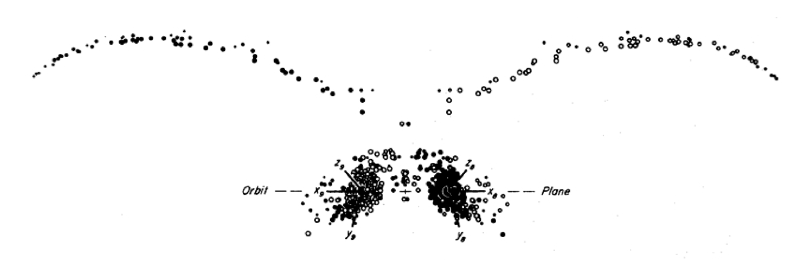
\includegraphics[width=0.8\textwidth]{Toomre.eps}
    \includegraphics[width=0.8\textwidth]{Antennae.eps}
    \caption[Early simulation of Antennae Galaxies]{The simulations of
    \citet{Toomre1972} showed how the kinematics of galaxy mergers can produce
    the variety of tidal structures seen in objects like the Antennae galaxies.
    The top image shows the result of one of the \citet{Toomre1972} simulations.
    \textit{Image credit: Adapted from figure 23 of \citet{Toomre1972}}
    The bottom image shows an observation of the actual object itself, the
    Antennae galaxies NGC 4038/4039. \textit{Image credit: NOAO/AURA/NSF, B.
    Twardy, B. Twardy, and A. Block (NOAO)}}
\end{figure}

The earliest numerical simulations of galaxy formation focused on the effects of
gravity alone.  A classic example of this are the simulations presented in
\citet{Toomre1972}, which showed that the irregular structures seen in galaxies
like NGC 4676 (``The Mice'') or NGC4038/4039 (``The Antennae Galaxies'') are the
results of major mergers between two disc galaxies, as is clear from figure 1.2.
These simulations used discs composed of a mere 120 test particles, and ignored
the effects of self-gravity between these particles.  Despite their crudeness,
these simulations showed that the morphologies of galactic bridges and tails could be
formed by the tidal interactions of two passing/merging galaxies.  The IBM
360/95 that \citet{Toomre1972} (with an inflation-adjusted purchase price in the
millions of dollars) used for their simulations was capable of 5.5 million
instructions per second, roughly $0.2\%$ the speed of a \$35 Raspberry Pi 3
available today.

Modern galaxy simulations do far more than merely integrate the equations of
motion for a few hundred test particles in a gravitational field.  Today, state
of the art simulations will track gravity (including self-gravity) for stars,
gas, and dark matter \citep{Aarseth1980,Stadel2001,Dehnen2002}; evolve Euler's
equations for the hydrodynamics of gaseous baryons
\citep{Wadsley2004,Teyssier2002,Bryan2014}; include models for radiative cooling
of gas that allow for cooling from both hydrogen and metal lines
\citep{Marri2003,Shen2010}; form stars from dense gas
\citep{Katz1992,Agertz2015}; and include models for feedback from massive stars
and black holes \citep{Katz1992,Springel2003,DiMatteo2005}.  These feedback
models have been the focus of much research in the past decade, as we shall
discuss further in this work.  Simulations also include treatments
for radiative transfer \citep{Gendelev2012,Krumholz2013} and
magneto-hydrodynamics \citep{Girichidis2015} as well.

Numerical modeling of galaxies is a difficult problem, as it involves processes
that take place over scales (both spatial and temporal) that span many orders of
magnitude.  This means that simulations will always be unable to resolve at
least some fraction of the physics taking place within the galaxy.  For this,
carefully designed ``sub-grid'' models are required to include the macroscopic
effects that unresolvable microscopic processes yield. 

\subsection{Gravity}
Gravity is typically solved using algorithms designed to minimize the workload
that would be needed for a direct summation of each particle or grid cell
($\mathcal{O}(N^2)$ for N grid cells/particles).  This becomes intractable for
larger numbers of resolution elements, as the workload will scale as the sixth
power of the linear resolution (an order of magnitude better linear resolution
will be $10^6$ times more expensive!).  In order to reduce these costs,
algorithms have been developed that allow for more efficient gravitational
force calculations.  Tree-based methods \citep{Barnes1986} reduce the
computational cost of long-ranged (and thus less significant) force
calculations by using space-partitioning trees.  Short-range force calculations
are done particle-by-particle, while long-range forces are calculated against
larger tree cells, thus reducing the cost of calculating gravity to
$\mathcal{O}(N\log N)$.  Particle-Particle/Particle-Mesh ($P^3M$) methods
\citep{Couchman1991} produce similar scalings, but rather than using a
spatial tree rely on a spectral Fourier-based approach to calculate long-ranged
interactions.  Recently, the Fast Multipole Method \citep{Greengard1987} has
been applied to the calculation of gravitational forces
\citep{Dehnen2002,Hahn2013} using a multipole expansion of Green's functions.
This allows for extremely efficient gravity calculation, scaling linearly with
particle number ($\mathcal{O}(N)$).  This method allows it to now be possible to
run N-body simulations with greater than $10^{12}$ particles\citep{Potter2016}.

\subsection{Hydrodynamics}
Hydrodynamical solvers usually come in one of two classes: Eulerian or
Lagrangian.  Eulerian methods discretize space into fixed volume elements with
fixed boundaries.  By breaking a simulation volume into a grid of cells that
each contains scalar and vector quantities those quantities can be advected
between cells according to the solver scheme.  Eulerian schemes typically allow
for higher-order solvers, lower intrinsic noise, and better resolved shocks
(when at rest relative to the grid) \citep{Teyssier2002,Stone2008,Bryan2014}.
They suffer from intrinsic mixing and diffusion that scales with the flow
velocity relative to the grid, poor integration of circular orbits, and costly
timestep limits \citep{Agertz2007,Tasker2008}.  A variety of Eulerian solvers
exist, ranging from the staggered mesh, high-order upwind \& artificial
viscosity scheme ZEUS, used in codes such as {\sc ENZO}
\citep{Stone1999,Bryan2014}, to the 2nd order Godunov method MUSCL used by {\sc
ramses} \citep{vanLeer1976,Teyssier2002}, or the 3rd order PPM scheme of {\sc
Athena} \citep{Stone2008}.  Lagrangian methods instead discretize mass, breaking
the volume into discrete points, each of which moves at the fluid
velocity to advect the quantities it contains, with smoothing functions used to
interpolate values in between particles; hence the name for the most common
Lagrangian method, Smoothed Particle Hydrodynamics (SPH).  Lagrangian methods
couple easily to tree and particle-mesh codes for gravity calculation, are
Galilean invariant, and intrinsically conserve mass, energy, and momentum
(linear and angular) \citep{Katz1996,Wadsley2004,Springel2005}.  The perfect
conservation of angular momentum is critical for accurately tracking orbits. SPH
methods typically use artificial viscosity to handle shocks, and as such have
difficulty in capturing subsonic turbulence \citep{Bauer2012}.  Recently, new
methods have begin to extend the basic SPH method using higher order gradient
estimates that are allowing accuracy on subsonic tests that rival the best
Eulerian schemes \citep{Springel2010,Hopkins2015,Valdarnini2016}. 

Modern galaxy simulations also now use a variety of strategies for judiciously
applying computational power where it is most needed.  Eulerian methods will
commonly use \textit{Adaptive Mesh Refinement} to increase resolution in regions
of interest (typically where gas is densest).  Lagrangian methods automatically
do this, as a denser region definitionally must contain more fluid elements.  

\subsection{Designing Simulations}
Beyond the choice of algorithms, the construction of appropriate inital
conditions is also important.  To study large populations of galaxies, along
with large-scale structure, large-volume cosmological boxes with volumes
$\gtrsim 10^6\;\rm{Mpc^3}$, but with spatial resolutions $\sim \rm{kpc}$ are
used (for example, the {\it Illustris} simulations have a softening length of
$1.4\;\rm{kpc}$ \citealt{Vogelsberger2014b}).  Studying how individual galaxies
form is typically done with cosmological zoom simulations, where a comparatively
cheap dark-matter only simulation is first run to select a region of interest,
which is then resimulated with higher resolution and baryonic physics included
\citep{Navarro1993}. Zoom-in simulations can typically achieve an order of
magnitude or better resolution than full cosmological boxes.  A number of groups
today are using these zoom-in simulations to study the impact of feedback
processes over cosmic time \citep{Stinson2013,Hopkins2014,Agertz2015}.  Isolated
galaxy disc simulations use a constructed disc profiles containing gas and
stars, embedded within a dark halo. These cannot show how galaxies form in a
cosmological environment, but can be run with $\sim \rm{pc}$ resolution to study
closely how internal processes within a galaxy take place
\citep{Hopkins2011,Benincasa2016}.  Details of these internal processes are
discussed in section 1.3.

The earliest attempt to track the formation of a galaxy in a cosmological
context with the effects of star formation and feedback included was by
\citet{Katz1992}.  This simulation used the Lagrangian TREESPH 
\citep{Hernquist1989} to evolve a volume of gas and dark matter from an initial
linear perturbation, including small-scale power derived from CDM predictions
\citep{Zeldovich1970,Peebles1982}.  Gas was allowed to cool radiatively using
rates calculated for primordial gas.  This study introduced a model for star
formation that is still the standard for most simulations of galaxy formation.
Observations \citep{Kennicutt1998} have suggested that the star formation rate
is a power law of the gas density: $\dot\Sigma_*\propto\Sigma_{gas}^\alpha$, with
$\alpha=1-2$.  If it is assumed that gas collapses to form stars in some
multiple $c_*$ of its freefall time \citep{Schmidt1959}, $t_{ff}$, a simple
3-dimensional star formation model can be built with the form:
\begin{equation}
    \dot\rho_* = \frac{c_*\rho_{gas}}{t_{ff}} = c_*\sqrt{\frac{\rho^3_{gas}}{4\pi G}}
\end{equation}
\citet{Katz1992} used a $c_*$ parameter of $0.1$, which is within the range of
what is typically used in simulations today ($1-100\%$).  On top of the model
for star formation, feedback was included without the use of any significant
subgrid model:  $10^{51}\;\rm{erg/SN}$ worth of energy was injected back into
the ISM by smoothing it over a number of resolution elements.  One of the key
findings of \citet{Katz1992} was that the vast majority of SN energy was
radiated away, making them very ineffective at regulating star formation within
the galaxy.  In the end, \citet{Katz1992} found that the peak star formation in
the simulated galaxy was nearly 10 times greater than in observed galaxies.
\citet{Thacker2000} later showed that the smoothing of energy used by
\citet{Katz1992} resulted in a large overestimation of the cooling rates in
feedback-heated gas. Since then, much work has gone into developing models for
feedback that address the issue of overcooling that was present in these
earlier simulations.  These efforts will be described in detail in the next
section.

\section{The Importance of Feedback}\label{intro:fb}
\begin{figure}
    \includegraphics[width=\textwidth]{M82.eps}
	\caption[Massive outflows in M82]{The evidence for feedback is no clearer
	than here in the Cigar Galaxy, M82.  The Hubble Space Telescope reveals massive
	outflows of hot ionized gas through the red $H\alpha$ emission as gas is
	blasted out of the galaxy in a bipolar flow. \textit{Image credit: NASA, ESA
	and the Hubble Heritage Team STScI/AURA}}
\end{figure}
Evidence has been building for decades that galaxy and star formation is not a
one way process of gravitational collapse.  A number of internal processes can
release a tremendous amount of energy back into the ISM of the galaxy, stirring
or even ejecting that gas.  Analytic calculations that omit feedback processes
found that gas should rapidly collapse into the smallest halos that can cool
radiatively (halos with a virial temperature of $\sim 10^4\;K$, or a mass of
$\sim10^8\Msun$).  This leads to an overproduction of stars in small galaxies at
high redshift (the ``cooling catastrophe'') \citep{Cole2001,Benson2003}.  The
observational signatures of feedback are abundant.  Lyman $\alpha$ forest
observations probing the intergalactic medium (IGM) have found that the IGM is
polluted with metal ions at great distances from any galaxies
\citep{Sargent1988,Songaila1996,Dave1998}.  These metals must have been ejected
by galactic outflows from the ISM of galaxies where they formed. Figure 1.3
shows a composite image of the dwarf starburst M82, where fast, massive outflows
have been seen leaving the ISM.  These outflows have been observed as a
ubiquitous feature of starburst galaxies and quasar host galaxies
\citep{Veilleux2005,Werk2014}.  Numerical models also have pointed towards
feedback as an essential ingrediant in forming both realistic galaxies and the
structures within them. Simulated galaxies develop unrealistically compact
morphologies without feedback \citep{Stinson2006}.  Inside of the galaxy,
simulations of individual molecular clouds have star formation rates an order of
magnitude too high \citep{Agertz2013} when feedback is omitted.  Clearly,
if we wish to accurately simulate galaxies, we must also accurately model the
feedback processes that shape those galaxies.

The two primary sources of feedback energy are massive stars and SMBHs.  Massive
stars ($M>5M_\odot$) experience short, violent lives.  Prior to their death,
they will drive fast $v>1000\;\rm{km/s}$ stellar winds \citep{Weaver1977}, and
ionize their surrounding gas with UV radiation \citep{Krumholz2009}.  At the end
of their lives, $4-30\;\rm{Myr}$ later, these stars die in energetic
core-collapse SN, liberating $\sim10^{51}\;\rm{erg}$
\citep{Wilson1985,Bethe1990}.  Figure 1.4 shows the total budget of available
energy liberated by a population of stars with a standard \citet{Chabrier2003}
IMF.  The total energy released by a population of stars with solar metallicity is
$\sim 2\times10^{51}\;\rm{erg/M_\odot}$.  Most of this energy is released as
photons, over the lifetime of each star.  These will both couple weakly with the
ISM, depositing little energy, and only heat gas to a relatively modest
temperature, much cooler than the virial temperature for galaxies like our own.
While stellar winds from a cluster will have comparable luminosity to
supernovae, two factors limit the effectiveness of these winds at driving
galaxy-scale outflows.  First, because these stellar winds are produced early,
they couple to the dense environment of the cluster's natal cloud, resulting in
orders of magnitude shorter cooling times for the hot bubbles they drive.
Second, the vast majority of the energy liberated in stellar winds comes from
the most massive stars, that die within $4\Myr$, giving stellar winds a total
energy budget of $10\%$ of the supernovae budget \citet{Leitherer1999}.
This means that supernovae, despite only contributing $\sim1\%$ of the total
energy released by a stellar population, may have the greatest impact on
galactic scales.  This energy imparts heat and momentum to the surrounding ISM,
and can accelerate cosmic rays in the shocks that result \citep{Bell1978}.  In
galaxies with actively growing SMBHs, the accretion disc that forms as gas
funnels into the black hole can reach temperatures exceeding $10^9\;\rm{K}$
through viscous heating \citep{Antonucci1993}.  This makes these accretion discs
some of the most luminous objects in the universe, and can heat the gas that
surrounds the galaxy to choke off the accretion of gas onto the galaxy, shutting
off star formation.

\begin{figure}
    \includegraphics[width=0.8\textwidth]{FB_budget.ps}
    \caption[Stellar feedback energy budget]{Most of the energy released by a
    stellar population comes from the luminosity of the stars within that
    population.  Despite this, because supernovae couple more easily to the ISM,
    it is believed they have the greatest effect on galactic scales.  The data
    shown here was produced with {\sc starburst99} \citep{Leitherer1999}}
\end{figure}

The coupling of feedback energy to the ISM is what determines the effectiveness
of that feedback.  In the lowest mass galaxies, UV photoheating may be the
primary regulator of star formation \citep{Efstathiou1992}.    However, UV
radiation has characteristic temperatures too low to drive galactic winds.
Large {\sc Hii} regions, such as 30 Doradus, have observed expansion rates of
only $25\;\rm{km/s}$ \citep{Chu1994}, far below the velocities needed to drive
galaxy-scale outflows.  Radiation pressure on dust grains has been suggested as
a driving mechanism for outflows \citep{Murray2011}.  Simulations that see a
large effect from radiation-driven galactic winds have thus far relied on major approximations
\citep{Roskar2014,Agertz2015} and questionably large infrared optical depths
\citep{Hopkins2014}.  Without high optical depths and multiple scattering, UV
photons will be reprocessed to IR that escape before imparting significant
energy or momentum to the surrounding gas \citep{Dale2005,Walch2012,Krumholz2013}.

On top of releasing just $10\%$ of the energy released by supernovae, stellar
winds are active during the early stages of a massive star's life.   Simulations
of molecular clouds with feedback from star clusters
\citep{Gendelev2012,Rogers2013} have found that most stellar wind energy is
expended disrupting the molecular clouds the clusters live in.  While these
winds (along with radiation pressure and UV-heated gas) do not significantly
escape the cluster, the channels they open within the cloud allow a large
fraction of SN energy to escape the dense molecular environment, while the
energy from winds and radiation are expended in disrupting the cloud.  Thus, for
galaxy-scale simulations that do not resolve the internal structure of
individual molecular clouds, the effects of UV radiation and stellar winds can
be safely omitted.

On the galactic scale, feedback regulates star formation in two primary ways.
Energy and momentum deposited into the ISM can heat and disrupt the cool clouds
of gas which form stars \citep{Rogers2013}, and increase the ISM scale height to
limit the formation of cool clouds out of the warm ISM
\citep{Ostriker2010,Benincasa2016}.  If that feedback is vigorous enough, gas
can actually be ejected from the disc into the circumgalactic medium (CGM)
\citep{Larson1974,Heckman1987,Hopkins2012b}.  Even if this material is still
bound to the halo, it can take $\sim\;\rm{Gyr}$ to return to the ISM.  This
limits star formation by simply removing the fuel for the process.  These
outflows are needed to explain observations of low star formation efficiencies
in massive galaxies \citep{Behroozi2013,Moster2013}, observations of outflowing
gas \citep{Lynds1963,Heckman1987}, a metal-polluted intergalactic medium
\citep{Shen2010}, and the low bulge fraction in star forming galaxies
\citep{Brook2012}.  In order to see how the local deposition of feedback energy
drives these winds, simulations with realistic models for hot stellar feedback
are required.

\subsection{Numerical Challenges for Hot Feedback}
The greatest difficulty with including the effects of feedback in simulations of
galaxy evolution is the combination of extreme gradients of temperature,
density, and velocity all in a relatively small mass/volume.  Without
overwhelmingly high resolution, hot feedback gas will be numerically mixed with
cold ISM, often resulting in gas with relatively high density and temperatures
of $\sim10^5\;\rm{K}$, where radiative cooling times are extremely short.  This
results in feedback energy being completely lost due to radiative cooling, as
was first seen by \citet{Katz1992}.  Indeed, as \citet{Thacker2000} showed, how
feedback energy is deposited into the ISM has a huge impact on whether that
feedback has any effect.  This problem has been tackled using a few different
strategies.  

Since overcooling is the problem, many models have attacked this directly by
either temporarily disabling cooling \citep{Thacker2000,Stinson2006} or
depositing feedback energy into a second, nonthermal energy component
\citep{Agertz2013}.  While this does limit radiative losses, it produces gas
that exists in an unphysical region of the $\rho-T$ phase diagram.  This gas may
lack the high temperatures and velocities required to actually escape the disc.
It also has the potential to introduce an \textit{undercooling} problem as
resolution becomes higher and feedback-heated gas becomes resolvable.
Alternatively, energy may be injected not as heat, but as momentum, which
naturally does not cool
\citep{Navarro1993,Mihos1994,Scannapieco2006,DallaVecchia2008,Dubois2008}.
Unfortunately, this adds the additional complexity of momentum cancellation (how
to treat neighbouring stars/clusters, where two stars are depositing momentum
with opposing directions), and if this momentum results in strong shocks, these
shocks will convert the momentum back into thermal energy that can radiate
away the very energy the model is designed to preserve \citep{Durier2012}.
This often means kinetic/momentum feedback models must be combined with
hydrodynamic decoupling that renders feedback-heated gas into a form that does
not interact with the surrounding ISM \citep{Springel2003,Vogelsberger2013}.
Naturally, this makes outflow properties strongly influenced by numerical
choices \citep{DallaVecchia2008}.  A third choice is to stochastically deposit
feedback energy only when enough energy is available to produce gas temperatures
high enough for cooling times to be short \citep{DallaVecchia2012,Crain2015}.
In these models, SN events are effectively grouped together, somewhat decoupling
feedback spatially from star formation.  The choice of temperature to heat gas
to is a purely numerical parameter, and can dramatically change the
effectiveness of these models.  Finally, some \citep{Springel2003,Murante2015}
attempt to directly address the unphysical numerical mixing of hot and cold gas
by separating the two phases and tracking each component separately.  This
completely solves the overcooling problem, and allows the two components to cool
radiatively.   Unfortunately, it also means that cold star-forming gas is
permanently coupled to hot feedback-heated gas: preventing the simulation of  a
resolved multiphase ISM, and effectively making the cold/warm ISM an anchor
holding down potential hot outflows.  This means these multiphase models have to
be coupled with parameterized models to capture outflows \citep{Springel2003}.
Often, these simple models simply choose a fraction of feedback energy to be
deposited as kinetic ``kicks'' to a some gas particles.  Like other kinetic
feedback models, this is frequently combined with hydrodynamical decouplings
\citep{Vogelsberger2013}.

All of these models attempt to solve the problem of overcooling with unphysical
approximations: disabled cooling, hydrodynamic decoupling, stochastic deposition
of feedback energy, and imposed multiphase ISM models.  These choices make it
difficult to understand what details of simulated galaxy evolution are a result
of these numerical free parameters, as opposed to the actual physics of
self-regulated star formation and SN-driven outflows.  What is needed is a model
that captures the effects of feedback while matching as closely as possible the
actual physical processes involved below the resolution scale.  Simulations that
rely on complex, numerically-motivated subgrid models are devoid of serious
predictive power.  When the results obtained depend heavily of the tuning of
multiple free parameters, those results can at best probe one point in the space
of the possible, rather than hew away at that space to discover the region of
the probable, and ultimately, the truth.  

\subsection{Superbubbles: The Natural Scale for Feedback}
The formation of massive stars takes place mostly in clusters of $10^4$ or more
stars.  This means that the SN of these stars can be treated not as individual
dumps of $10^{51}\;\rm{erg/SN}$, but instead as a luminosity of
$10^{34}\;\rm{\frac{erg}{s \cdot M_\odot}}$.  This allows us to use stellar wind
models like those of \citet{Weaver1977} to study the evolution of superbubbles driven by
hot stellar feedback processes, like SN or stellar winds.  Each individual SN's
ejecta thermalizes in a small region within the center of the bubble, and the
resulting hot gas drives a shock that sweeps up the surrounding ISM.  In a short
time, the swept-up ISM can radiatively cool efficiently resulting in a thin,
cold shell surrounding a hot, diffuse bubble.

The structure and evolution of superbubbles have been the subject of a great
deal of analytic study.  \citet{Castor1975} found that the time evolution of
superbubbles has a similarity solution, similar to the \citet{Sedov1959}
adiabatic blast wave solution: 
\begin{equation}
    R(t)=27n_0^{-1/5}L_{36}^{1/5}t_6^{3/5}\;\rm{pc} 
\end{equation}
\begin{equation}
    V(t)=16n_0^{-1/5}L_{36}^{1/5}t_6^{-2/5}\;\rm{km/s}
\end{equation}
$n_0$ is the ambient density in $\rm{cm^{-3}}$, $L_{36}$ is the luminosity of
the star cluster in $10^{36}\;\rm{erg/s}$, and $t_6$ is the time in
$10^6\;\rm{yr}$.  The evolution of hot mass in the bubble, and the effects of
cooling in the swept-up shell, were examined in \citet{Weaver1977}.  The
\citet{Weaver1977} results were extended to clustered SN by \citet{MacLow1988}.
They calculated that the typical cooling time for the hot bubble was
$\sim15\;\rm{Myr}$, with a weak dependence on the total luminosity and ambient
density.  Before significant cooling can occur in the hot interior, $\sim35\%$
of the total feedback luminosity is lost to cooling of the swept-up shell, which
cools in $\sim10^4\;\rm{yr}$.  This means that, rather than the $1-10\%$ of
energy preserved from a single supernova blast \citep{Chevalier1974}, $\sim65\%$
of the initial energy budget is retained in the kinetic energy of the cold shell
and thermal energy of the hot interior.  \citet{MacLow1988} also demonstrated
that, as superbubbles do not have surface tension, they are not depressurized by
cold clouds, and instead simply deform around them while continuing to expand.
\citet{Silich1996} studied the effects of an ISM permeated with cold clumps in
greater detail, finding that the general behaviour discussed in
\citet{MacLow1988} held even in the case of an inhomogeneous ISM.  Even with
$50\%$ of the ISM mass trapped in cold clouds (which penetrate the cold shell of
the superbubble), the total hot mass within the superbubble will only vary by
$\sim20\%$.

A key insight in these studies was that hot bubbles would evaporate their cold
shell through thermal conduction.  In a hot ionized plasma, electrons are able
to penetrate temperature gradients and deposit energy within cooler material.
This produces a pressure gradient that establishes a mass flux against the
temperature gradient, evaporating the cold shell into the hot bubble.  This
evaporation means that a hot bubble with temperature $T$ and radius $R$ gains
mass at a rate of:
\begin{equation}
    \frac{{\rm d }M_b}{{\rm d}t} = \frac{16\pi\mu}{25k_B} CT^{5/2}R
\end{equation}
Where $C$ is the Spitzer conduction coefficient,
$C=6\times10^{-7}\;\rm{erg\;s^{-1}\;cm^{-1}\;K^{7/2}}$, and $\mu$ is the mean
molecular weight of the gas in the bubble.  As the cold, evaporated material
acts to cool the hot bubble, this makes the bubble's interior temperature
self-regulating: higher temperatures give higher mass flux, cooling the bubble.
This acts to push interior bubble temperatures to $10^6-10^7\;\rm{K}$.

\citet{DallaVecchia2012} showed that the temperature of feedback-heated gas can
ultimately determine its effectiveness in driving outflows and regulating star
formation, even with constant feedback energy.  The self-regulating temperature
of superbubbles provides the natural mechanism for setting this temperature:
thermal evaporation.  By including the effects of thermal evaporation between
unresolved hot bubbles and the surrounding cool ISM, feedback energy can be
deposited into the correct amount of ISM mass, giving realistic temperatures,
densities, and cooling times for feedback-heated gas.  This superbubble feedback
model is described in detail, and applied to the problem of Milky Way-like
galaxy formation in the chapters that follow.

\section{This Work and Organization of Chapters}
In this thesis, I present a new sub-grid model for the feedback from massive
stars.  I use this new model to study the importance of well-modelled SN
feedback in the cosmological evolution of MW galaxies, and how that feedback can
drive the outflows that are key to forming physically realistic galaxies.  I
then turn to the question of SN-regulation at the peak of the star formation
efficiency, and examine whether the turnover in this efficiency seen by studies
such as \citet{Behroozi2013,Moster2013} can be attributed to SN feedback alone.
Finally, I apply the simulations generated during these investigations to
see whether SN-regulated galaxies formed in a $\Lambda CDM$ cosmological context
can match observed scaling relations of nearby disc galaxies.

Chapter 2 presents the new superbubble feedback model, and describes the
implementation of this model in the simulation code {\sc GASOLINE2} (Wadsley et
al. 2016, submitted).  I show a series of tests that demonstrate the model is
robust to resolution changes, insensitive to magnetic field strength (which
affects conduction rates), and able to handle cases involving unresolved ISM
structure.  Finally, I show that simulations of isolated dwarf and Milky Way
like disc galaxies regulate their star formation and drive efficient galactic
outflows with this new feedback model.

Chapter 3 applies the feedback model described in chapter 2 to a cosmological
simulation of a Milky Way like galaxy.  This allows us to see how galaxies like
the Milky Way assemble themselves by regulating the flow of gas into the disc,
ejecting material to prevent the formation of a central stellar bulge and slow
the formation of stars.  We compare this to the same simulation run with the
simpler \citet{Stinson2006} feedback model to reproduce the results of
\citet{Stinson2010}, which used the same initial conditions as this study.  We
use this to study how this new, physically motivated feedback model change prior
assumptions about the effectiveness of SN feedback.  We also examine how
SN-driven outflows remove the fuel for star formation and bulge growth to
produce a realistic, bulgeless disc galaxy.

Chapter 4 extends the results presented in chapter 3 by simulating an additional
17 cosmological galaxies, reproducing the McMaster Unbiased Galaxy Simulations
(MUGS) presented in \citet{Stinson2010} with updated hydrodynamics and the new
feedback model described in chapter 2.  This MUGS2 sample spans the peak of the
star formation efficiency found by abundance matching studies like
\citet{Moster2013}, and using it we are able to show that SN feedback is unable
to regulate galaxies more massive than the peak halo mass of $10^{12}\;M_\odot$.
By analyzing the outflow properties of these galaxies, we are able to determine
a global relation between the halo mass (or disc mass) and the outflow mass
loadings.  We examine how the mass loading of galactic outflows is set through
evaporation, and how the effective temperature determines the effectiveness of
these outflows at regulating the formation of the galaxies in the MUGS2 sample.

Chapter 5 uses the sample of galaxies developed in the previous chapter to
test whether recent observational results presented in \citet{McGaugh2016}
are consistent with $\Lambda CDM$.  The radial acceleration relation (RAR) seen in
the SPARC sample \citep{Lelli2016b} of observed rotationally supported galaxies
shows that the accelerations within these galaxies are tightly correlated 
with the accelerations due to baryons alone.  We show, using the sample of
galaxies generated in chapter 4, that this relation simply falls out of the
dissipative collapse of baryons in a collisionless dark matter halo.  We also
show that this result is independent of stellar feedback.  Despite the insensitivity
to feedback processes at $z=0$, we show that feedback does result in evolution
of the RAR with redshift, and predict that a different RAR would be observed if
a similar study to \citet{Lelli2016b} were done for high-redshift galaxies.

Finally, in chapter 6 we conclude with a discussion of how each of these results
together improve our understanding of SN-regulated star formation in the
formation of disc galaxies.  We discuss how the results presented here improve
the understanding developed in past research and its impact on the direction of
research in galaxy evolution theory.  We conclude with a discussion of the
future directions that this research points, and a number of open questions
raised by this research.

\bibliographystyle{mnras}
\bibliography{library}
